%%%%%%%%%%%%%%%%%%%%%%%%%%%%%%%%%%%%%%%%%
% Short Sectioned Assignment
% LaTeX Template
% Version 1.0 (5/5/12)
%
% This template has been downloaded from:
% http://www.LaTeXTemplates.com
%
% Original author:
% Frits Wenneker (http://www.howtotex.com)
%
% License:
% CC BY-NC-SA 3.0 (http://creativecommons.org/licenses/by-nc-sa/3.0/)
%
%%%%%%%%%%%%%%%%%%%%%%%%%%%%%%%%%%%%%%%%%

%----------------------------------------------------------------------------------------
%	PACKAGES AND OTHER DOCUMENT CONFIGURATIONS
%----------------------------------------------------------------------------------------

\documentclass[paper=a4, fontsize=11pt]{scrartcl} % A4 paper and 11pt font size

\usepackage[T1]{fontenc} % Use 8-bit encoding that has 256 glyphs
\usepackage{fourier} % Use the Adobe Utopia font for the document - comment this line to return to the LaTeX default
\usepackage[english]{babel} % English language/hyphenation
\usepackage{amsmath,amsfonts,amsthm} % Math packages
\usepackage{graphicx}
\usepackage{verbatim}

\usepackage{geometry}
\usepackage{float}

\usepackage{lipsum} % Used for inserting dummy 'Lorem ipsum' text into the template

\usepackage{sectsty} % Allows customizing section commands
\allsectionsfont{\centering \normalfont\scshape} % Make all sections centered, the default font and small caps

\usepackage{fancyhdr} % Custom headers and footers
\pagestyle{fancyplain} % Makes all pages in the document conform to the custom headers and footers
\fancyhead{} % No page header - if you want one, create it in the same way as the footers below
\fancyfoot[L]{} % Empty left footer
\fancyfoot[C]{} % Empty center footer
\fancyfoot[R]{\thepage} % Page numbering for right footer
\renewcommand{\headrulewidth}{0pt} % Remove header underlines
\renewcommand{\footrulewidth}{0pt} % Remove footer underlines
\setlength{\headheight}{13.6pt} % Customize the height of the header

\numberwithin{equation}{section} % Number equations within sections (i.e. 1.1, 1.2, 2.1, 2.2 instead of 1, 2, 3, 4)
\numberwithin{figure}{section} % Number figures within sections (i.e. 1.1, 1.2, 2.1, 2.2 instead of 1, 2, 3, 4)
\numberwithin{table}{section} % Number tables within sections (i.e. 1.1, 1.2, 2.1, 2.2 instead of 1, 2, 3, 4)

\setlength\parindent{0pt} % Removes all indentation from paragraphs - comment this line for an assignment with lots of text

\setlength{\parskip}{12pt}

%----------------------------------------------------------------------------------------
%	TITLE SECTION
%----------------------------------------------------------------------------------------

\newgeometry{top=0.4in, bottom=0.4in}

\newcommand{\horrule}[1]{\rule{\linewidth}{#1}} % Create horizontal rule command with 1 argument of height

\title{	
\normalfont \normalsize 
\textsc{University of Rochester\\CSC 249, Machine Vision\\Spring 2017} \\ [25pt] % Your university, school and/or department name(s)
\horrule{0.5pt} \\[0.4cm] % Thin top horizontal rule
\huge Homework 4 \\ % The assignment title
\horrule{2pt} \\[0.5cm] % Thick bottom horizontal rule
}

\author{Nathan Conroy} % Your name

\date{\normalsize\today} % Today's date or a custom date

\begin{document}

\maketitle % Print the title

%----------------------------------------------------------------------------------------
%	Part 1
%----------------------------------------------------------------------------------------

\section{Overview}

For this assignment, we were required to implement a Hough transform on an image that was provided to us in a previous homework assignment, as seen in Figure 1.1. Hough transform is a technique used for feature extraction such as detecting lines in an image. The process works by first creating an accumulator array representing the parameter space to store "votes" representing the features of the image as calculated by the algorithm, and then extracting the local maxima from the array to find the main features.

\begin{figure}[H]
  \centering
  \begin{minipage}[b]{0.45\textwidth}
    
\includegraphics[width=\textwidth]{original_image_binary.png}
    \caption{original image}
  \end{minipage}
\end{figure}

\restoregeometry

\section{Boundary Point Extraction}

The first step in my implementation of the algorithm involved extracting the boundary points from the original image. When using a Hough Transform to detect boundary lines in an image, this is a necessary step because the algorithm highlights lines of pixels that it finds in the image within the accumulator array. If the shapes were filled, the algorithm would find a surplus of lines in many directions within the shapes and instead of focusing on the edges it would instead focus on the most prominent line within the shape's body.

My algorithm for creating the image with the extracted boundary points was simple. I first created an array containing all zeros with the same dimensions as the original image. I then iterated through every pixel in the original image, and if it was not part of the background, I looked at every pixel within its 8-connected neighborhood. If any pixel in it's neighborhood was the background (pixel value 0), I set the corresponding pixel with the center of the neighborhood in the new array to value 255. The result was a binary image with just pixels representing the border of the components, as seen in Figure 2.1.

\begin{figure}[H]
  \centering
  \begin{minipage}[b]{0.45\textwidth}
    
\includegraphics[width=\textwidth]{extracted_boundary_points.png}
    \caption{original image with boundary point extraction}
  \end{minipage}
\end{figure}

\section{Hough Transform}

The first step in my implementation of the Hough Transform was creating the accumulator array. For the dimensions I decided to use 181 pixels for the width (representing degree values of 0 to 180), and height equivalent to the input image's height * width + 1, representing distance with a range from -(x + y) to (x+y) with an offset of x + y + 1. I chose this because it was a safe value that would work for all calculations because it is mathematically impossible for a value to fall outside of that range using the polar coordinate equation (r = x cos(theta) * y sin(theta)).

Once the accumulator array had been initialized, I then iterated through every pixel in the input image (the image with the extracted boundary points). If the pixel had a value greater than 0, meaning it isn't the background, I then iterated through every degree value from 0 to 180. Inside of that loop, I calculated the radian angle value from the degree value using the formula theta = degrees * (pi / 180), and the distance value using r = x cos(theta) + y sin(theta). I then went back to the accumulator array and incremented the value at position [ r + offset, degree + 1] by 1. At the end of the algorithm's run, the accumulator array represents the parameter space, which I displayed using imagesc and saved to the images folder. It can be seen in Figure 3.1. I applied a Gaussian low-pass filter to the parameter space image as well, seen in Figure 3.2. This was somewhat helpful with seeing the peaks of the image by reducing the noise.

Pre-computing the sin and cos values and using a lookup table would have been a good idea because it would have sped up my algorithm by avoiding having to calculate the values at every iteration. However, because the input image did not consist of many pixels, the runtime of my algorithm did not suffer much.

\begin{figure}[H]
  \centering
  \begin{minipage}[b]{0.9\textwidth}
    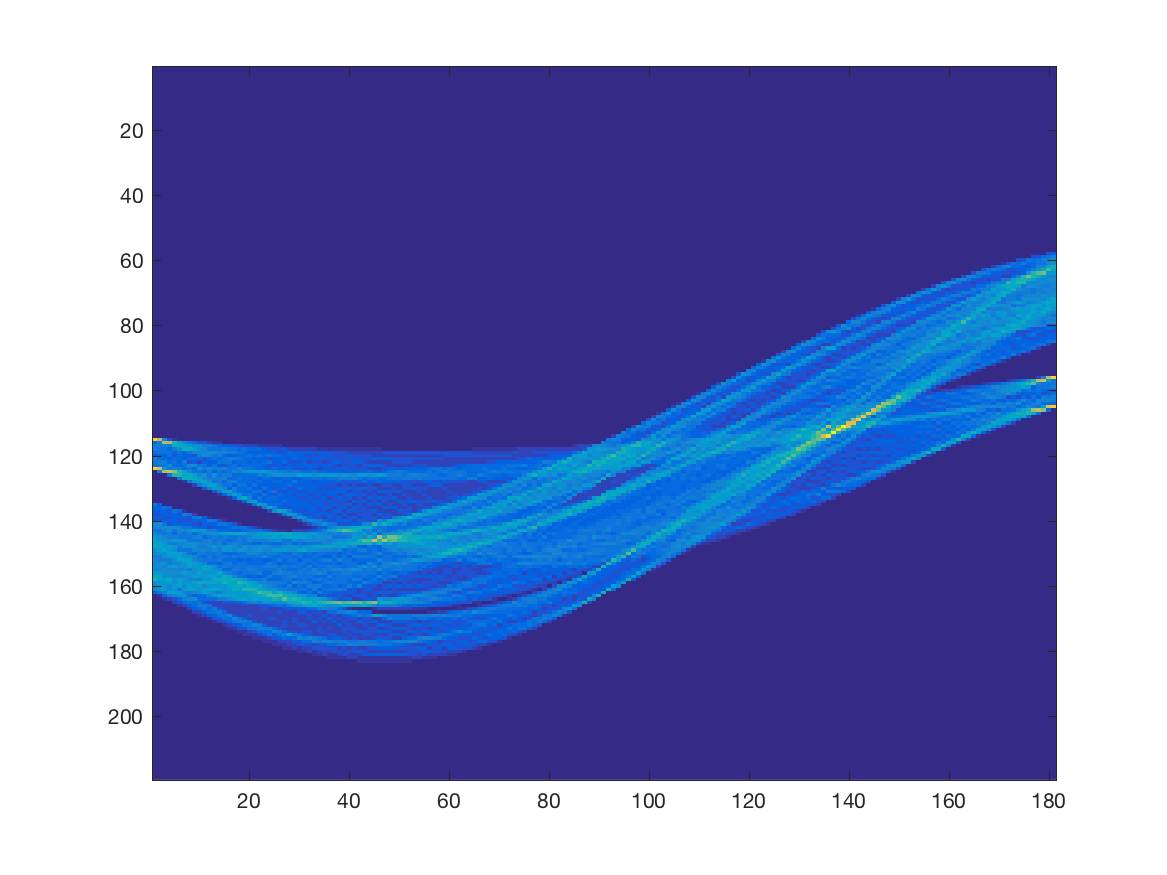
\includegraphics[width=\textwidth]{houghTransform_sc.png}
    \caption{parameter space image}
  \end{minipage}
\end{figure}

\begin{figure}[H]
  \centering
  \begin{minipage}[b]{0.9\textwidth}
    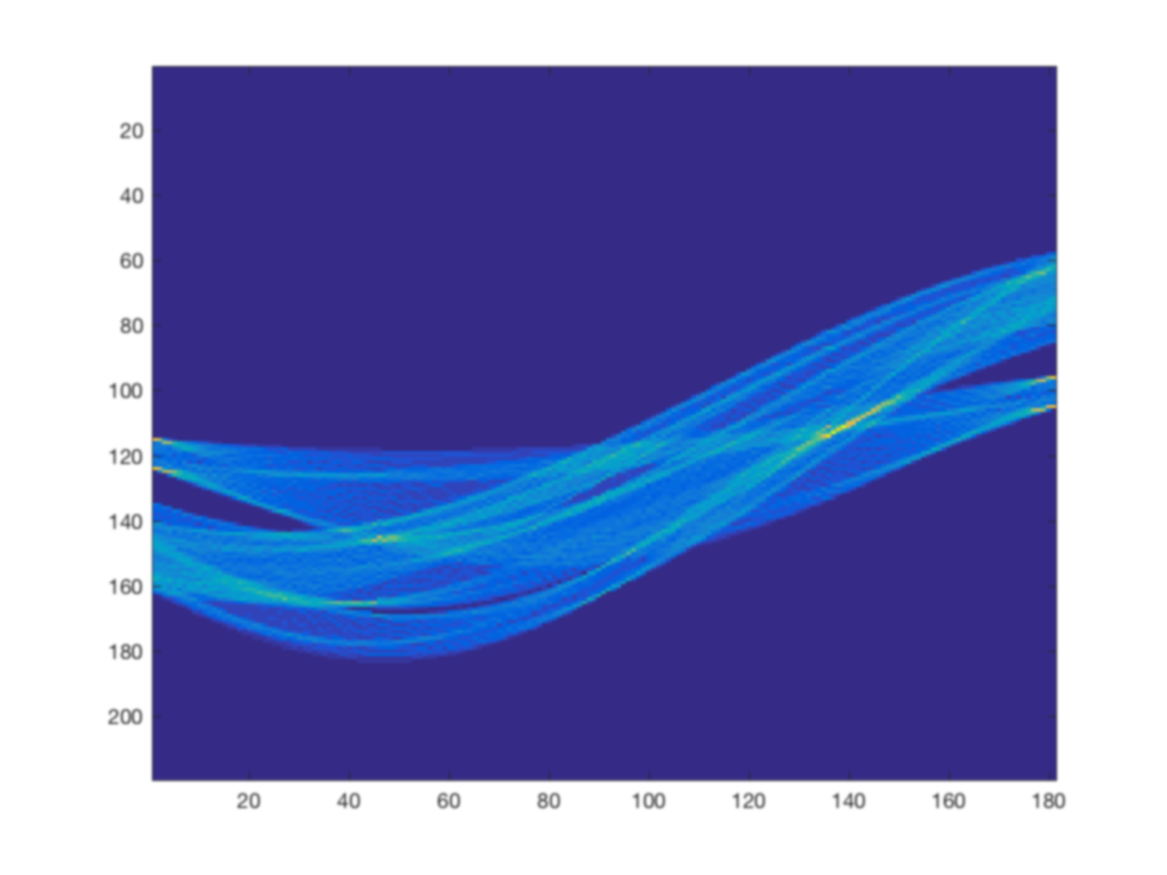
\includegraphics[width=\textwidth]{smoothed_image.png}
    \caption{smoothed parameter space image}
  \end{minipage}
\end{figure}

The brighter colors (red/yellow) in the image represent the highest values in the accumulator array. These pixels' indices represent common lines found in the image, and therefore the highest values represent the most prominent lines in the image. As you can see, these values are mostly at obvious intersection points between curves.

I extracted the peaks of these values at various thresholds and drew the lines found at these peaks on top of the input image in order to analyze the accuracy of the algorithm. The thresholds I used were vote counts of 30, 28, 25, 23, 20, and 18. Essentially, I cycled through the accumulator array and plotted any line using the polar coordinates specified by the array indices for any cell with a vote count at or above the threshold. The results of this proved to be fairly messy. The results can be seen in the figures below.

\begin{figure}[H]
  \centering
  \begin{minipage}[b]{0.49\textwidth}
    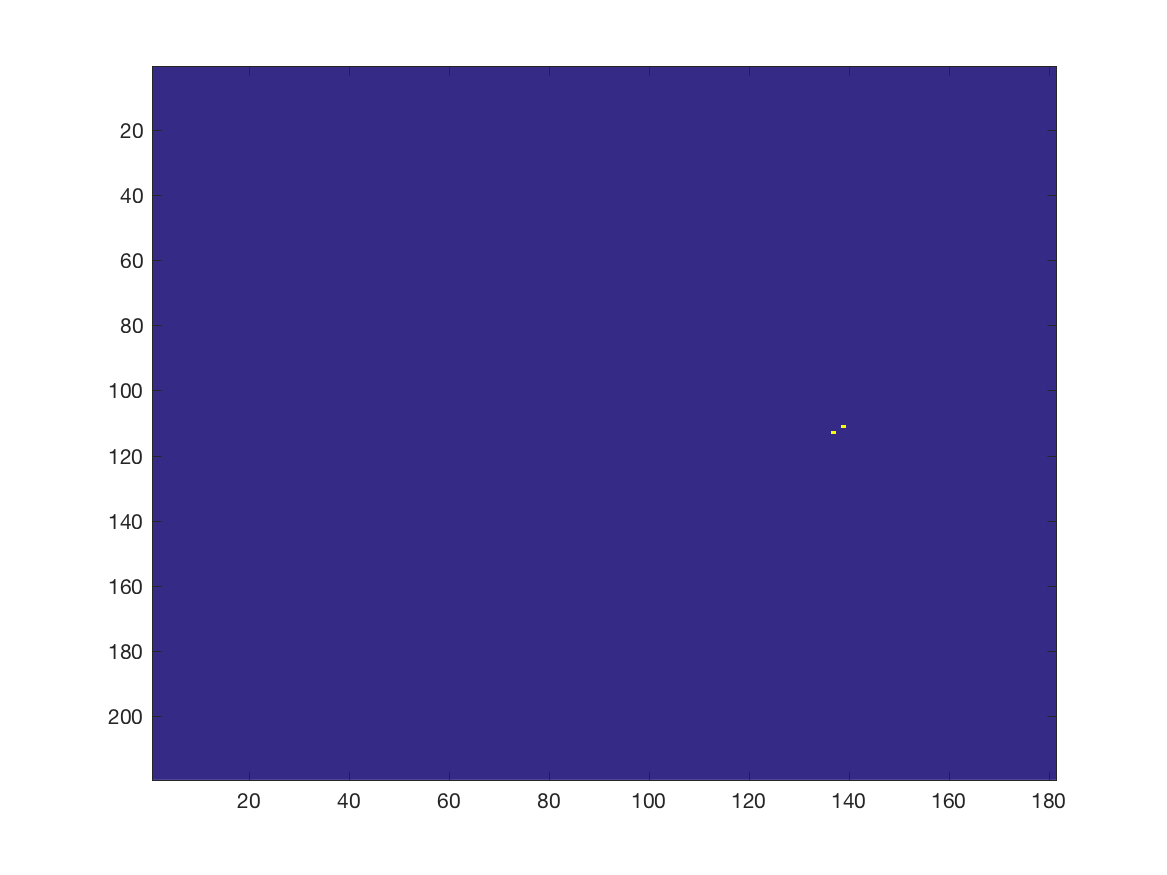
\includegraphics[width=\textwidth]{peaks_threshold_30.png}
    \caption{peaks, threshold = 30}
  \end{minipage}
  \hfill
  \begin{minipage}[b]{0.49\textwidth}
    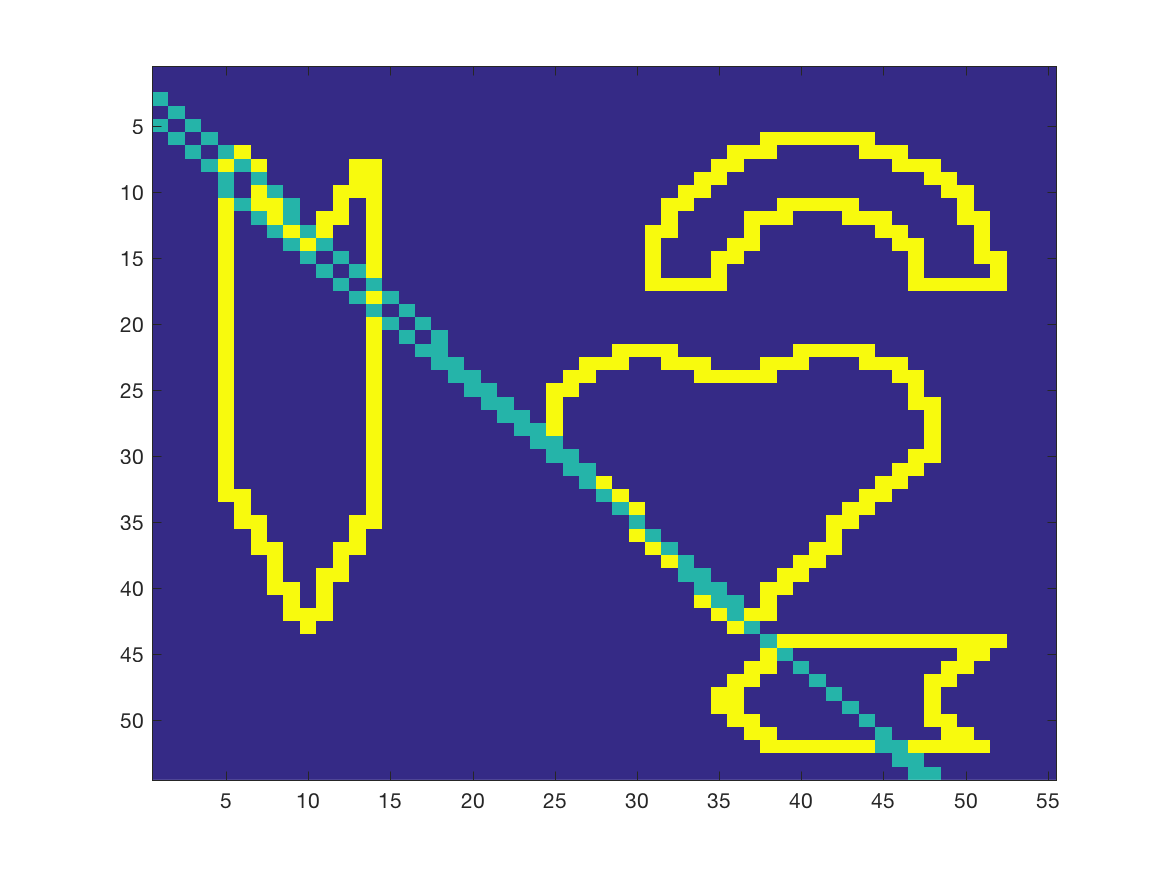
\includegraphics[width=\textwidth]{edgeDetection_threshold_30.png}
    \caption{detected lines, threshold = 30}
  \end{minipage}
\end{figure}

\begin{figure}[H]
  \centering
  \begin{minipage}[b]{0.49\textwidth}
    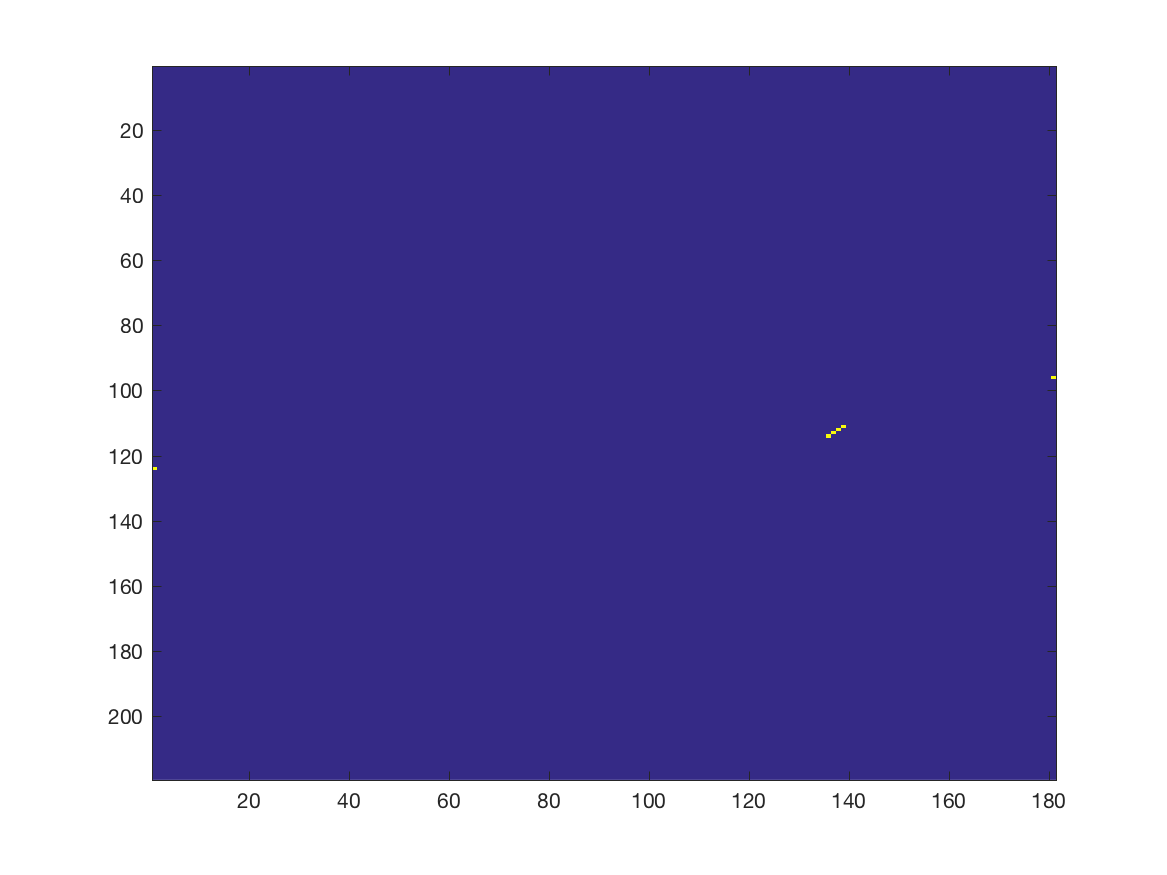
\includegraphics[width=\textwidth]{peaks_threshold_28.png}
    \caption{peaks, threshold = 28}
  \end{minipage}
  \hfill
  \begin{minipage}[b]{0.49\textwidth}
    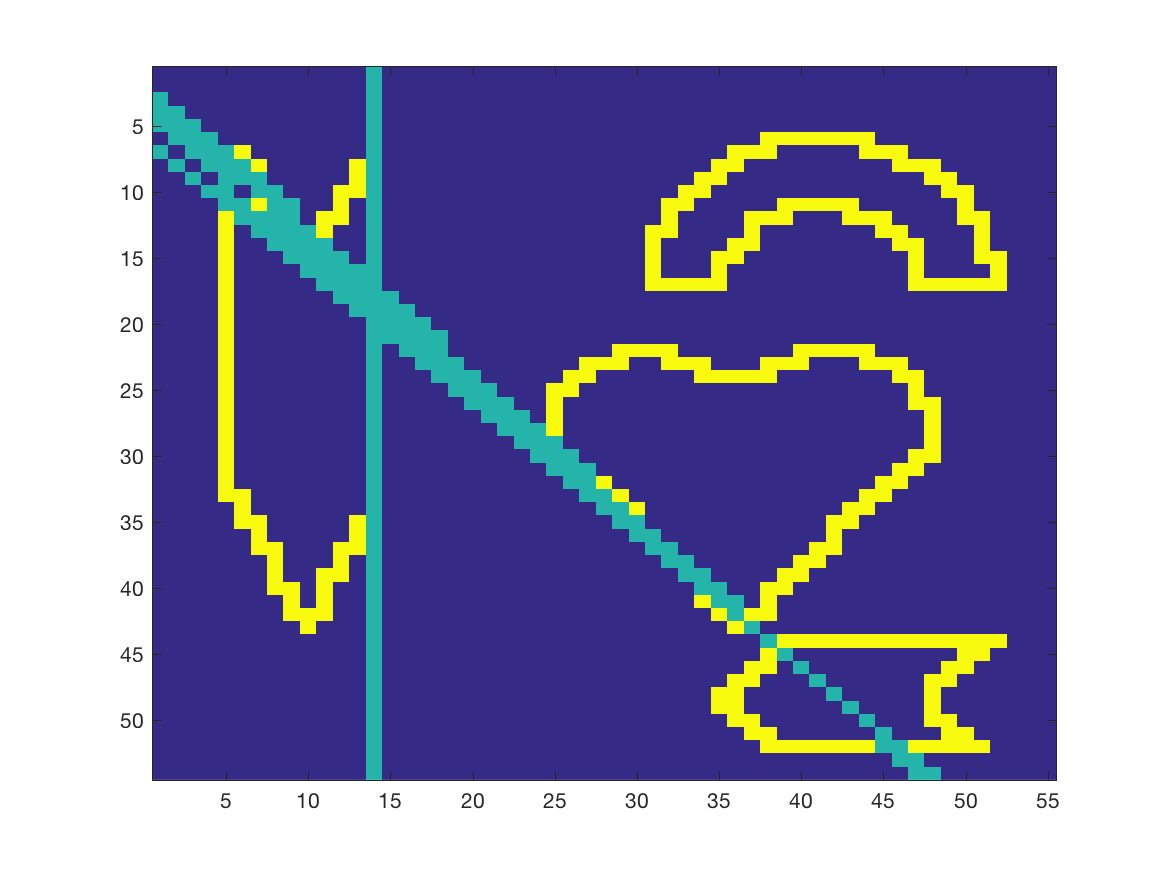
\includegraphics[width=\textwidth]{edgeDetection_threshold_28.png}
    \caption{detected lines, threshold = 28}
  \end{minipage}
\end{figure}

\begin{figure}[H]
  \centering
  \begin{minipage}[b]{0.49\textwidth}
    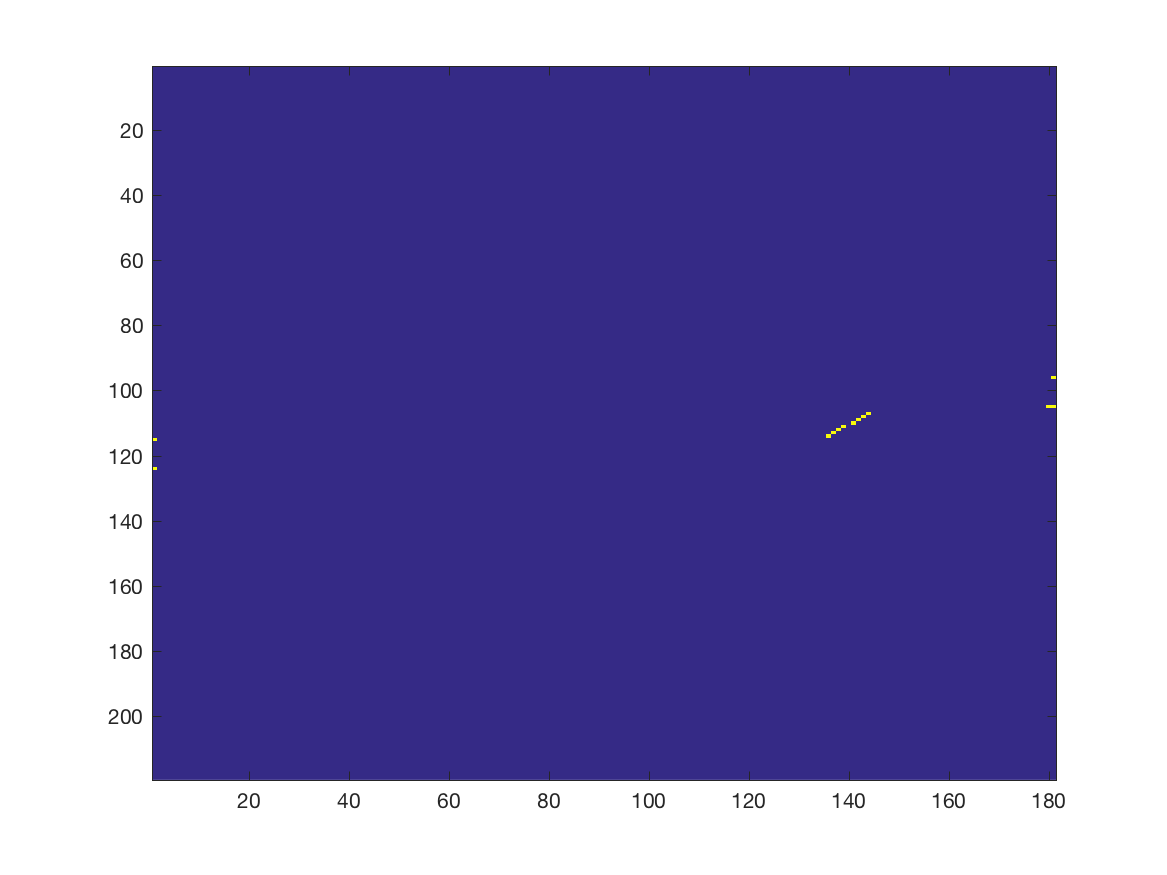
\includegraphics[width=\textwidth]{peaks_threshold_25.png}
    \caption{peaks, threshold = 25}
  \end{minipage}
  \hfill
  \begin{minipage}[b]{0.49\textwidth}
    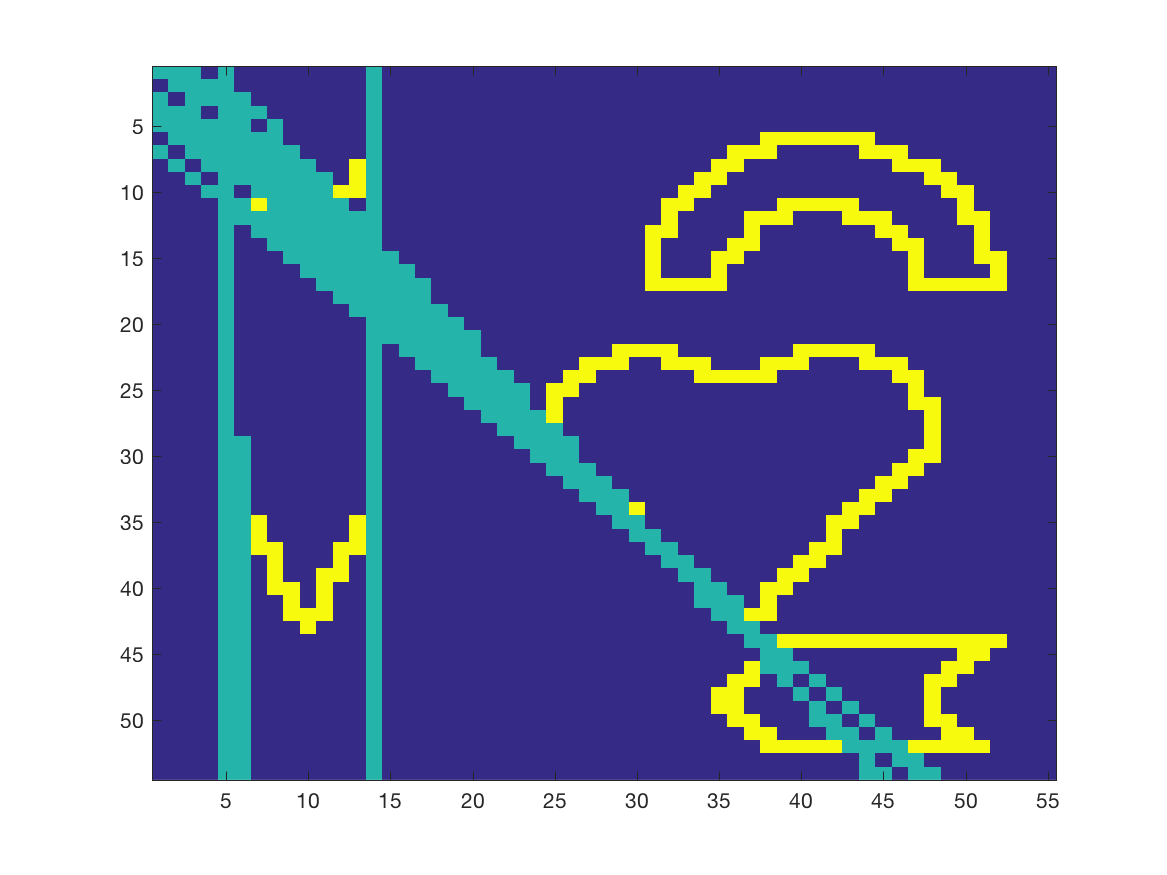
\includegraphics[width=\textwidth]{edgeDetection_threshold_25.png}
    \caption{detected lines, threshold = 25}
  \end{minipage}
\end{figure}

\begin{figure}[H]
  \centering
  \begin{minipage}[b]{0.49\textwidth}
    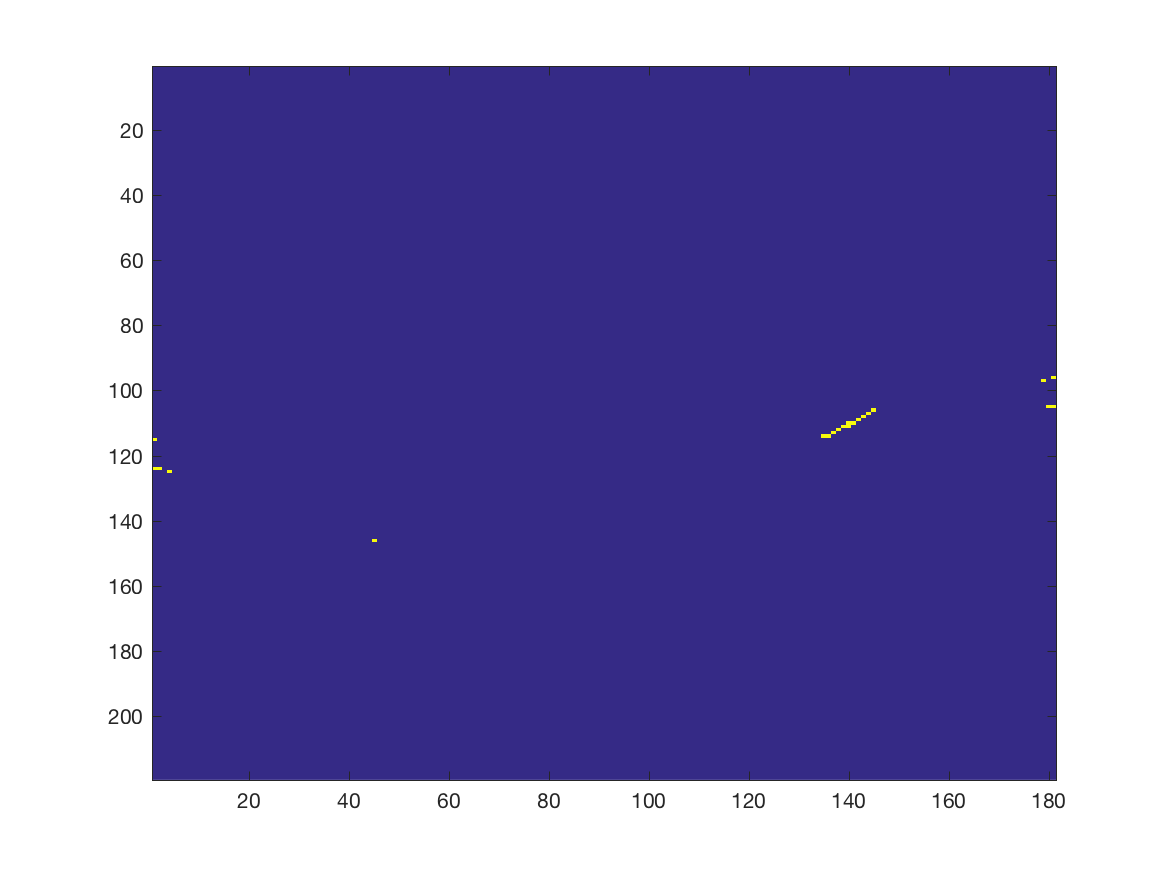
\includegraphics[width=\textwidth]{peaks_threshold_23.png}
    \caption{peaks, threshold = 23}
  \end{minipage}
  \hfill
  \begin{minipage}[b]{0.49\textwidth}
    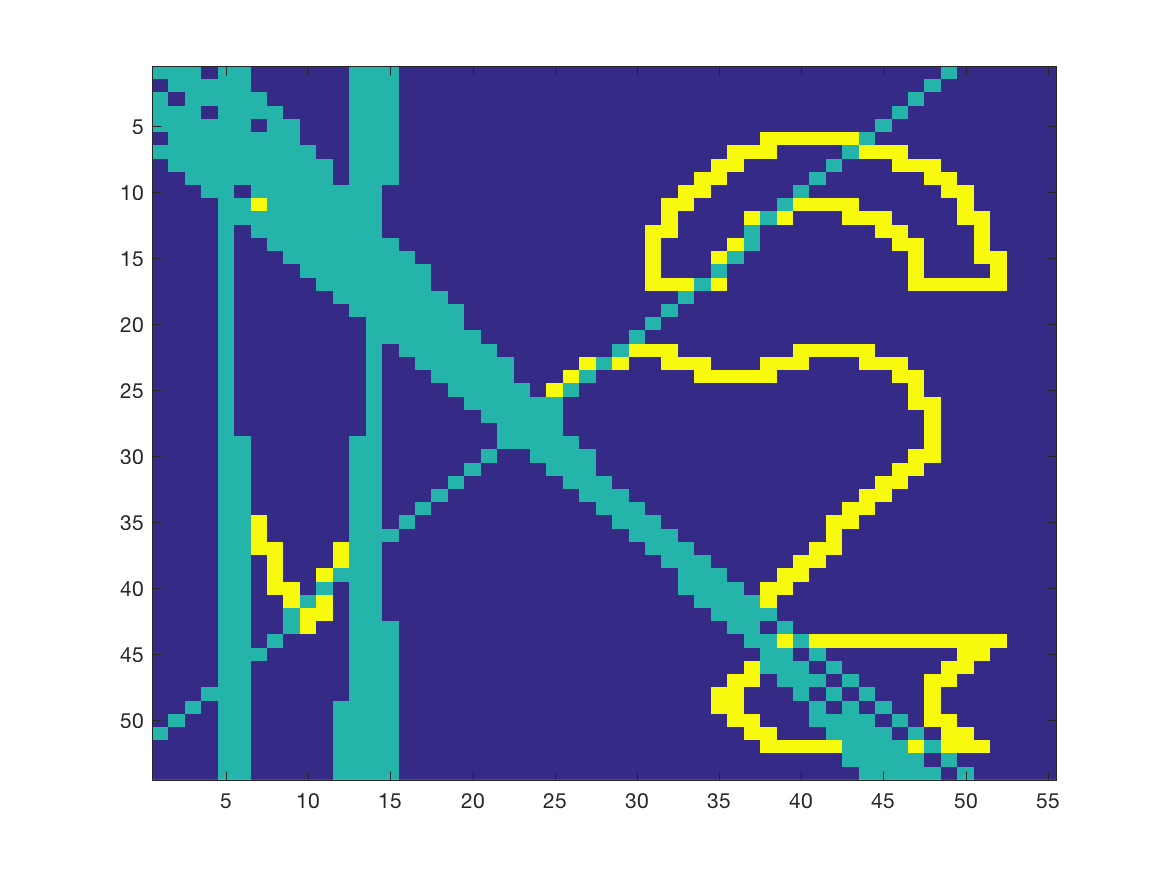
\includegraphics[width=\textwidth]{edgeDetection_threshold_23.png}
    \caption{detected lines, threshold = 23}
  \end{minipage}
\end{figure}

\begin{figure}[H]
  \centering
  \begin{minipage}[b]{0.49\textwidth}
    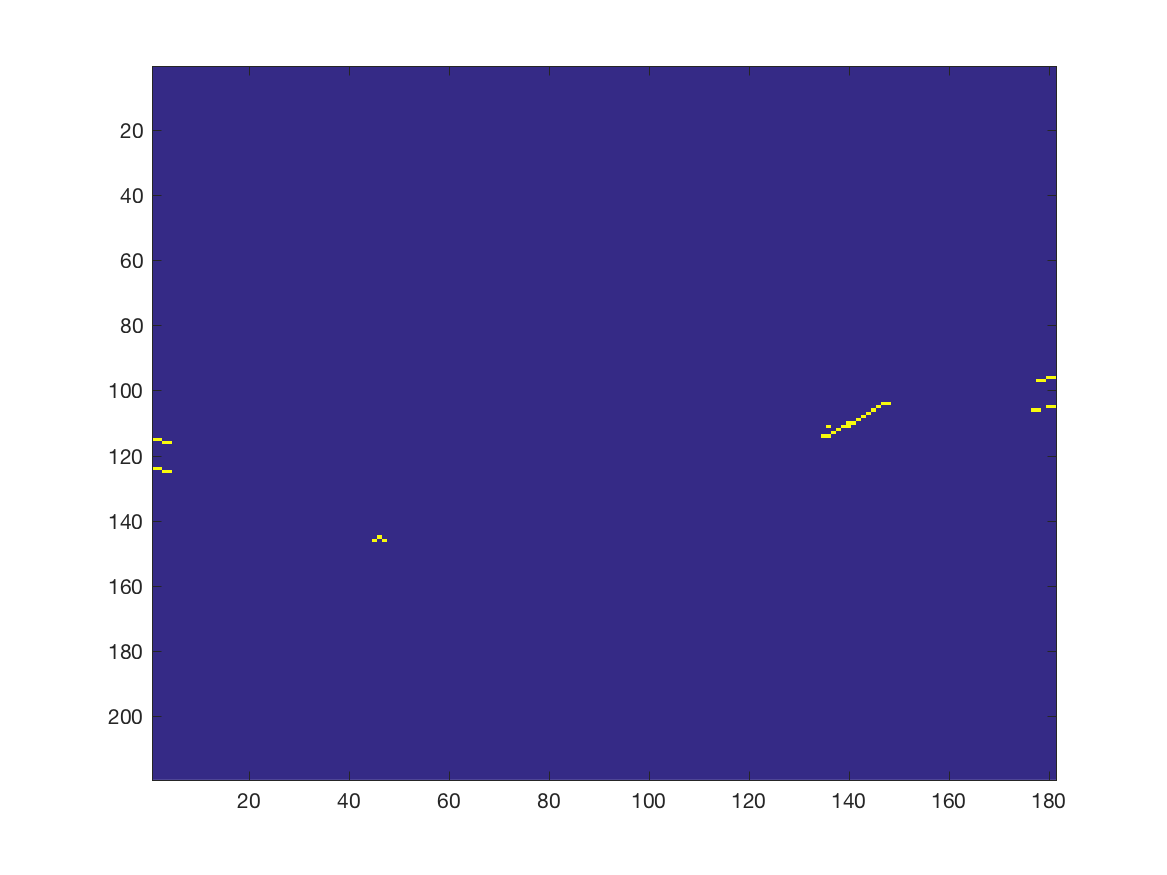
\includegraphics[width=\textwidth]{peaks_threshold_20.png}
    \caption{peaks, threshold = 20}
  \end{minipage}
  \hfill
  \begin{minipage}[b]{0.49\textwidth}
    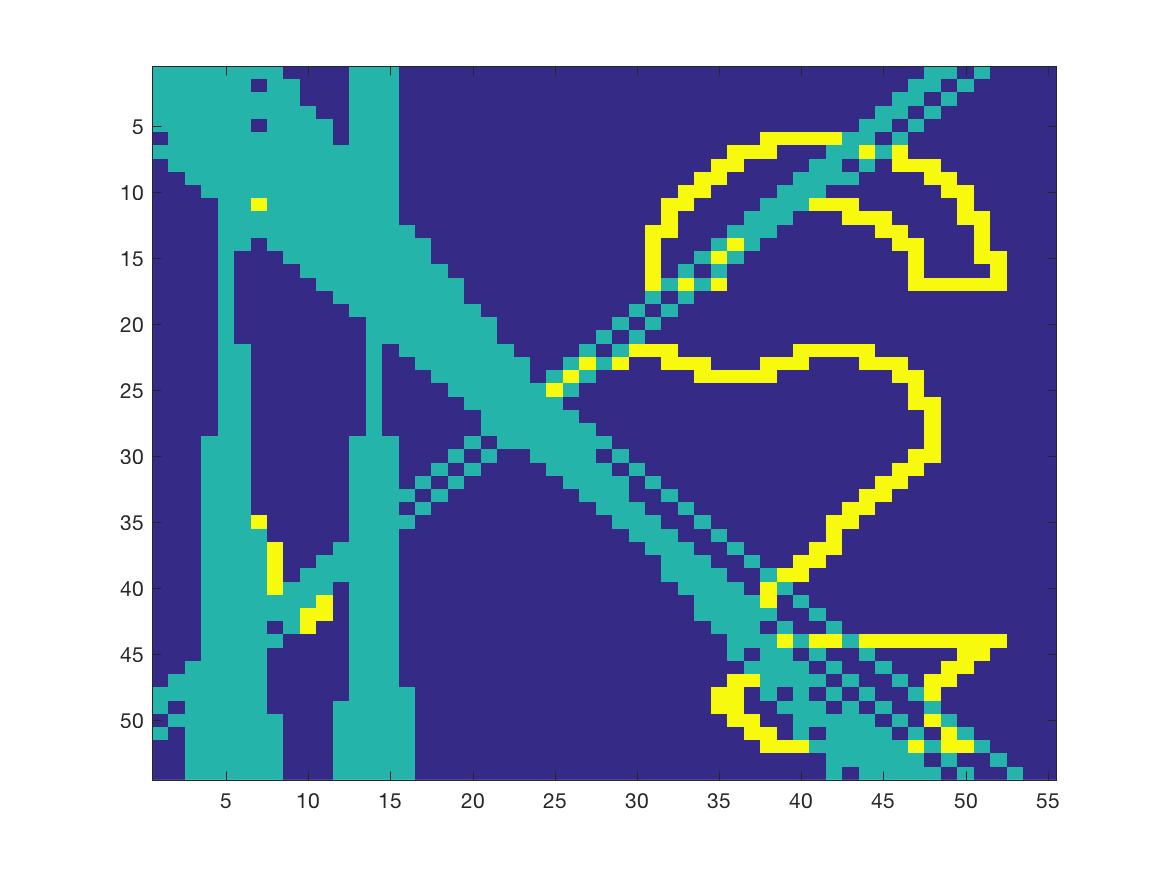
\includegraphics[width=\textwidth]{edgeDetection_threshold_20.png}
    \caption{detected lines, threshold = 20}
  \end{minipage}
\end{figure}

\begin{figure}[H]
  \centering
  \begin{minipage}[b]{0.49\textwidth}
    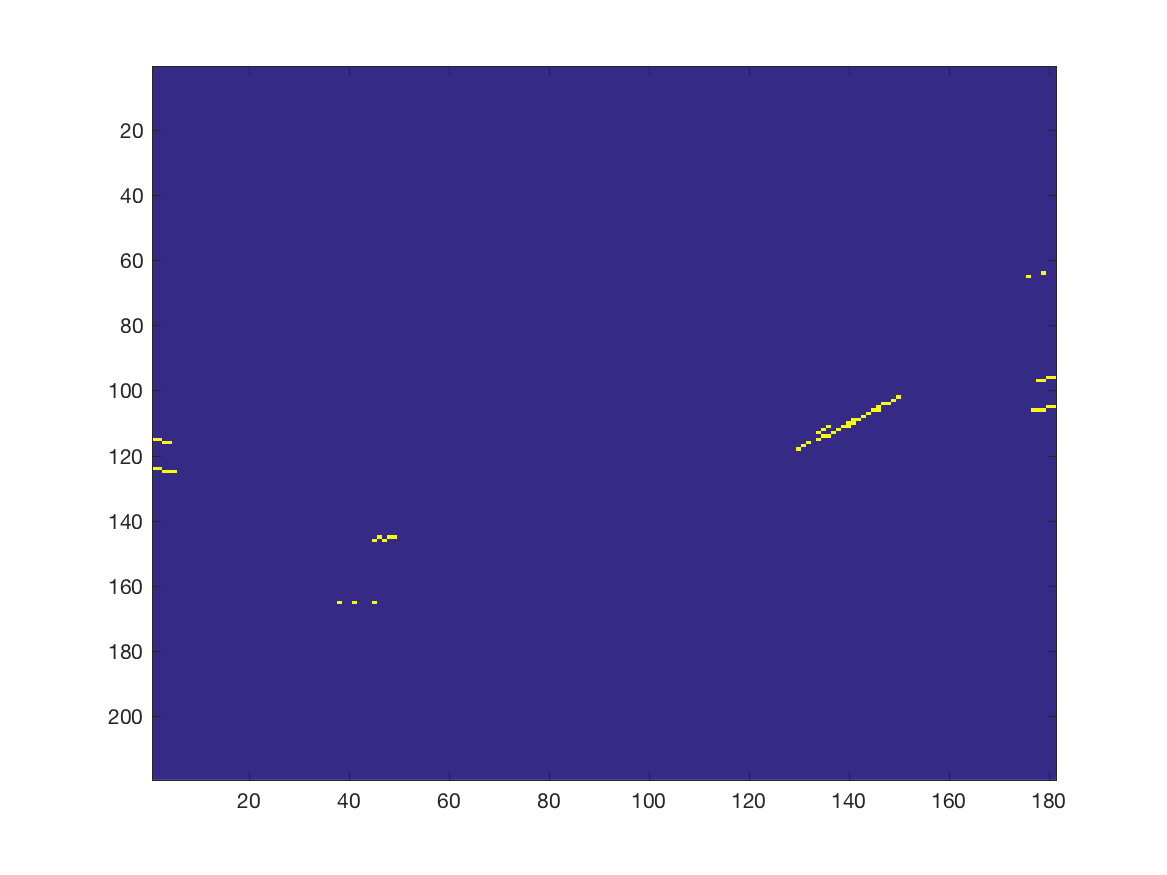
\includegraphics[width=\textwidth]{peaks_threshold_18.png}
    \caption{peaks, threshold = 18}
  \end{minipage}
  \hfill
  \begin{minipage}[b]{0.49\textwidth}
    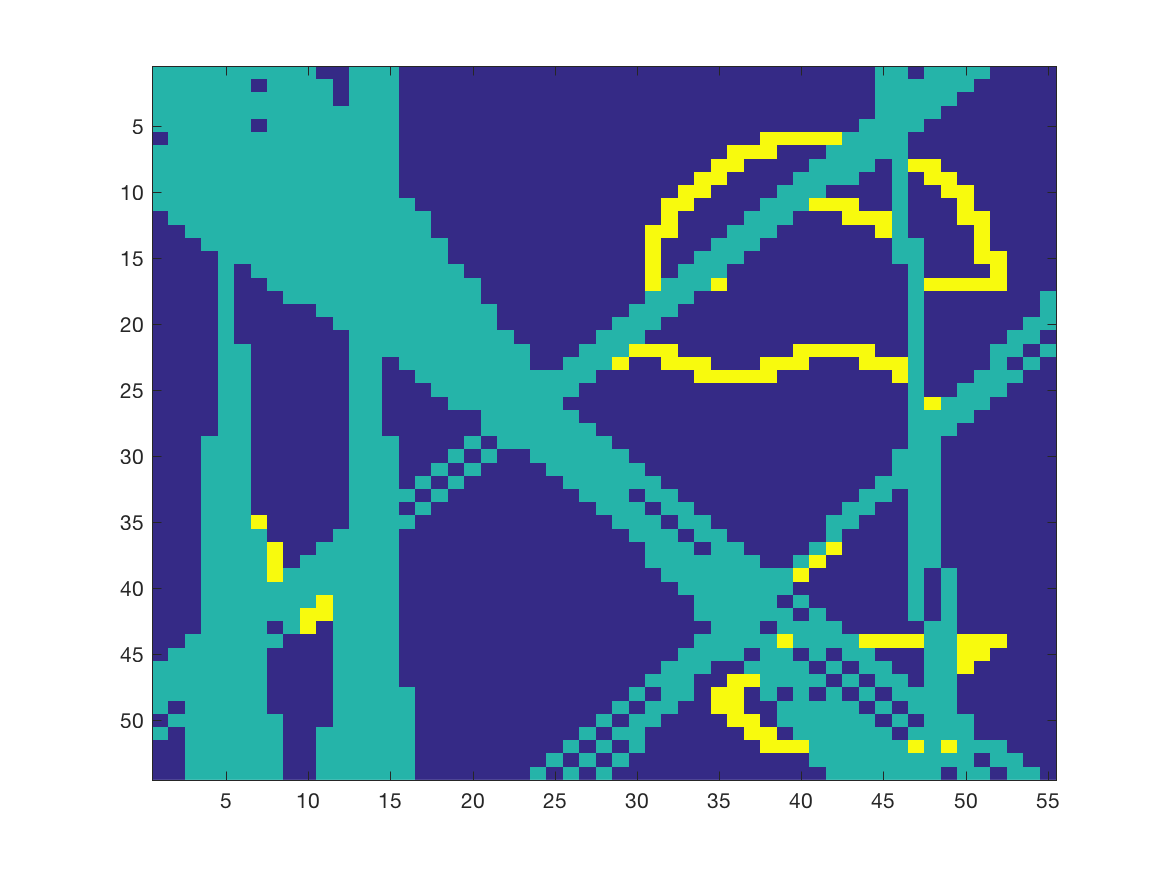
\includegraphics[width=\textwidth]{edgeDetection_threshold_18.png}
    \caption{detected lines, threshold = 18}
  \end{minipage}
\end{figure}

As I decreased the threshold, the detected lines became much more abundant, and the output image became very messy. This is because choosing a threshold is not a good way to decide what lines to plot simply because some regions have many cells with similar counts. A better way to handle this is to instead find the local maxima throughout the image, and only plot those values. I tested this by manually selecting the local maxima given by the parameter space image when the threshold was set to 18. The result of this trial was much cleaner, and showed the accuracy of the algorithm. It can be seen in Figure 3.15.

\begin{figure}[H]
  \centering
  \begin{minipage}[b]{0.75\textwidth}
    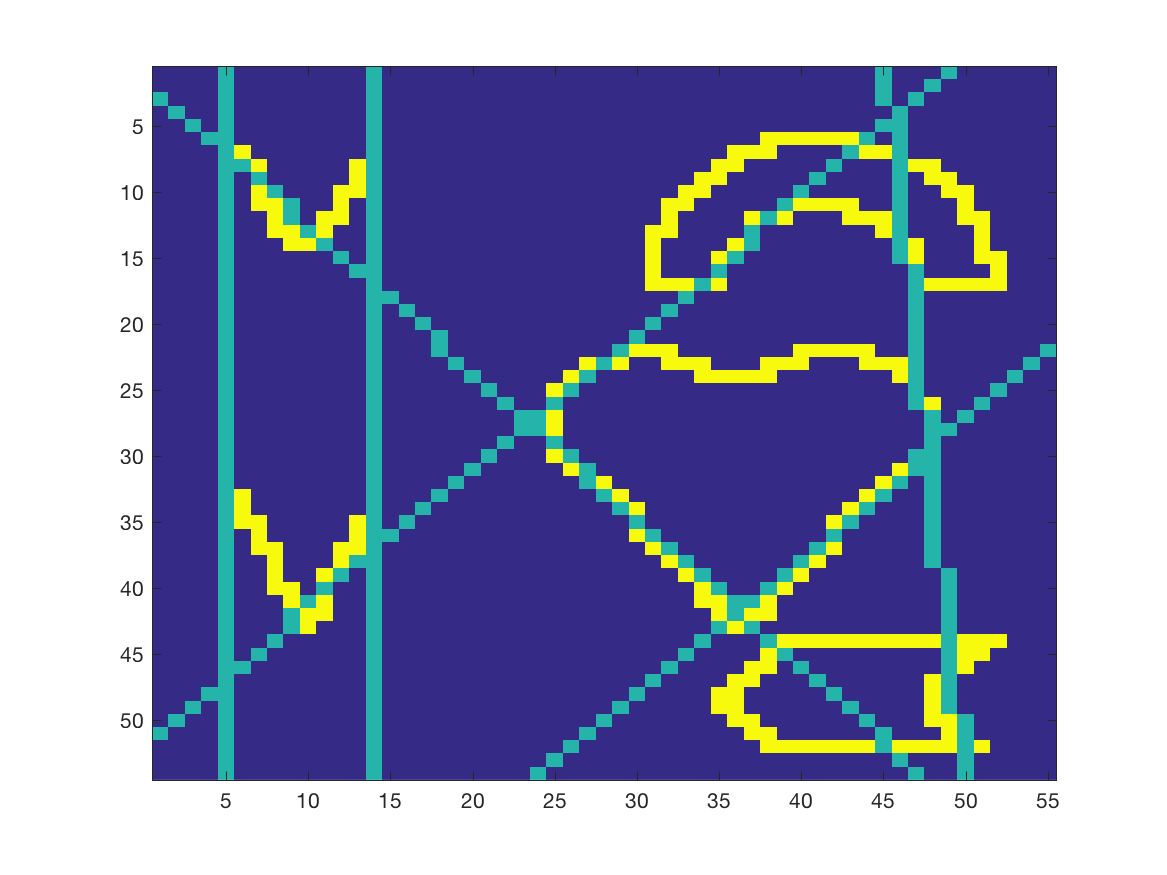
\includegraphics[width=\textwidth]{local_maxima_selection.png}
    \caption{line detection with local maxima, threshold = 18}
  \end{minipage}
\end{figure}

\section{Analysis}

Because the algorithm just finds the lines using distance and angle from the origin, it doesn't really give much insight to the length of each line. However, the lines associated with higher vote counts correspond to "lines" in the image containing the most pixels. Unfortunately, this does not account for line continuity. For example, if you look at the 2 lines detected when the vote count threshold was set to 30, they actually were made up of 3 smaller disconnected lines from 3 separate components in the input image. The largest continuous lines in the input image (the two vertical lines on the left side) were found when the vote count was between 25 - 30.

Note that polar representation, as I used in my implementation, is better than using the standard y = m x + b for computing Hough Transform. This is because of the way that vertical lines are represented. When using the standard form, the slope of a vertical line is infinite, and therefore would cause unbound values of the variable m.

\end{document}